\definecolor{gold}{rgb}{0.77,0.69,0.37}
\newlength{\hptitlewidth}
\newlength{\rationalh}
\newcommand{\hptitle}[2][\stockwidth]{%
\setlength{\hptitlewidth}{#1}%
\centering\color{white}%
\vskip 3cm\resizebox{.95\hptitlewidth}{!}{\textls[100]{HARRY POTTER AND THE}}%
\vskip 2mm%
\color{gold}%
\settoheight{\rationalh}{\resizebox{.95\hptitlewidth}{!}{\textls[20]{RATIONALITY}}}
\resizebox{!}{0.9\rationalh}{\textls[50]{METHODS}}%
\hfil\resizebox{!}{0.3\rationalh}{\textls[50]{Of}}%
\vskip 2mm%
\resizebox{.95\hptitlewidth}{!}{\textls[20]{RATIONALITY}}%
\vskip 8mm%
\color{white}%
\resizebox{.5\hptitlewidth}{!}{\textls[50]{\scshape{}Fanfiction by Eliezer Yudkowsky}}%
\vskip 4mm%
\resizebox{.35\hptitlewidth}{!}{\textls[50]{\scshape{}Deutsche Übersetzung}}%
\vfill%
\textls[50]{\scshape #2}%
\color{black}%
\vskip 1cm\ %
}
\providecommand{\fullvolumetitle}[1]{Buch #1: \volumetitle}

\ifcover%
\definecolor{backgroundcover}{HTML}{272c36}
\newpagecolor{backgroundcover}\afterpage{\restorepagecolor}
\newcommand\BackgroundPic{
\put(0,0){%
\parbox[b][\paperheight]{\paperwidth}{%
\vfill%
\centering%
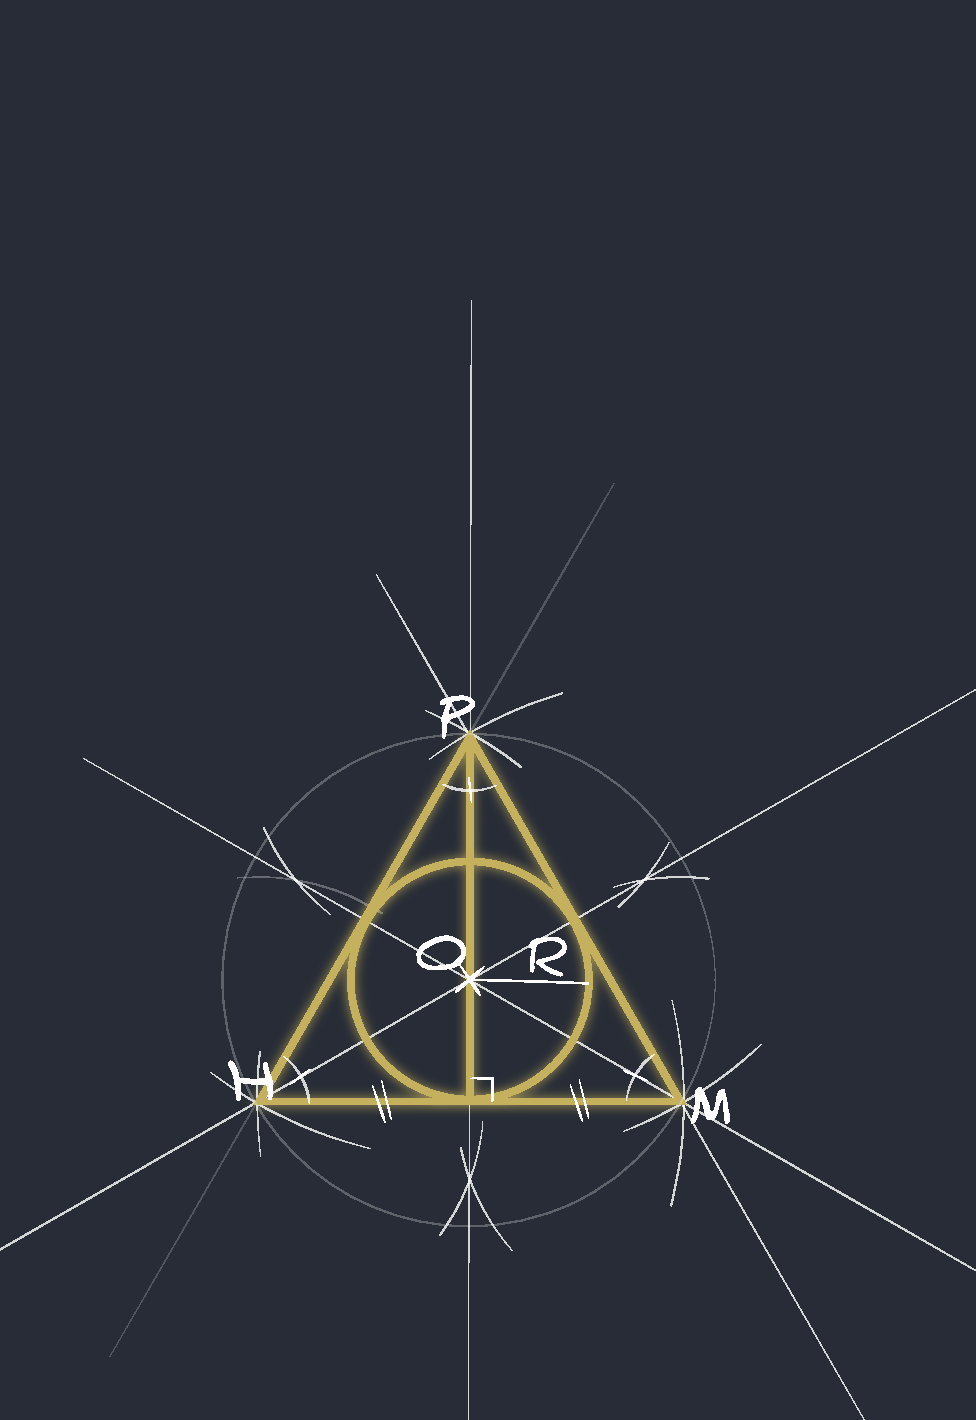
\includegraphics[width=\paperwidth,height=\paperheight,keepaspectratio]{cover1.pdf}%
\vfill%
}}}\AddToShipoutPicture*{\BackgroundPic}%
\AddToShipoutPicture*{\put(0,0){%
\parbox[b][\paperheight]{\paperwidth}{%
\hptitle{\fullvolumetitle{\volumenumber}}%
}}}%
\ %
\cleartorecto
\fi
\begin{center}
\thispagestyle{empty}
{\hpfont
\Huge\MakeUppercase{Harry Potter}\vspace*{0.5cm}

\Large\MakeUppercase{and the Methods of Rationality} %

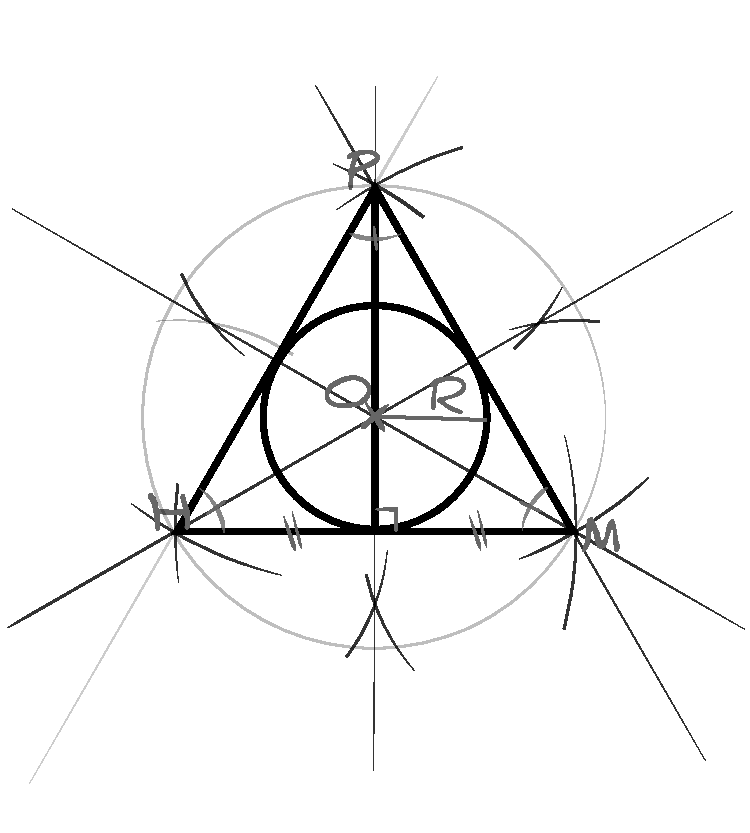
\includegraphics[scale=0.5]{bubble.pdf}

\vspace*{-1.0cm}
\Large Fanfiction by \vspace*{.25cm}

\huge \MakeUppercase{Eliezer Yudkowsky}%

\normalsize

\vspace*{1\baselineskip}
\fullvolumetitle{\volumenumber}
}

\vspace{0.7cm}

Basierend auf der Harry Potter Serie von J.~K.~Rowling\\
Author's disclaimer: J.~K.~Rowling owns Harry Potter, and no one owns the methods of rationality.
% Disclaimer: ~K.~Rowling besitzt alle Rechte an Harry Potter, aber niemandem gehören die Methods of Rationality.

~\\
Die englische Originalfassung gibt es auf \url{http://hpmor.com} als HTML und auf \url{https://github.com/rrthomas/hpmor/} als überarbeites PDF und eBook\\
~\\
% \vspace{0.7cm}
Das \href{https://github.com/entorb/hpmor-de/}{OpenSource Projekt} dieser deutschen Übersetzung auf\\
\url{https://github.com/entorb/hpmor-de/}
\\wird verwaltet von \href{https://entorb.net}{Torben Menke}


\end{center}

\newpage

